\chapter{Verwandte Arbeiten}\label{chapter:arbeiten}
In diesem Kapitel werden verwandte Arbeiten betrachtet, die sich mit der Forschungsfrage \glqq Wie lassen sich die Konzepte der Augmented Reality für den Bildungsbereich nutzen?\grqq{} oder einer angrenzenden Thematik beschäftigen. Dabei wird sowohl auf allgemeine Literatur, Studien, wissenschaftliche Arbeiten, als auch konkrete Anwendungen eingegangen und ihr Inhalt zusammengefasst.

\section{Augmented Reality in Education}
Das Buch \citep{geroimenko:ar-in-education} von \citeauthor{geroimenko:ar-in-education} beschäftigt sich mit dem Einsatz von Augmented Reality im Bildungsbereich. Im folgenden werden einmal die Grundaussagen des Buches zusammengefasst

\subsection{Aktueller Stand}
Smartphones stellen aufgrund des des Vorhandenseins verschiedener Software Development Kits (SDK) und ihrer Allgegenwart die aktuelle Hauptplattform für Augmented Reality dar. Während Head Mounted Displays vor allem an kleinere Zielgruppen und den professionellen Markt richten. \citep[Kapitel 1.2]{geroimenko:ar-in-education}\\
\begin{figure}
\centering
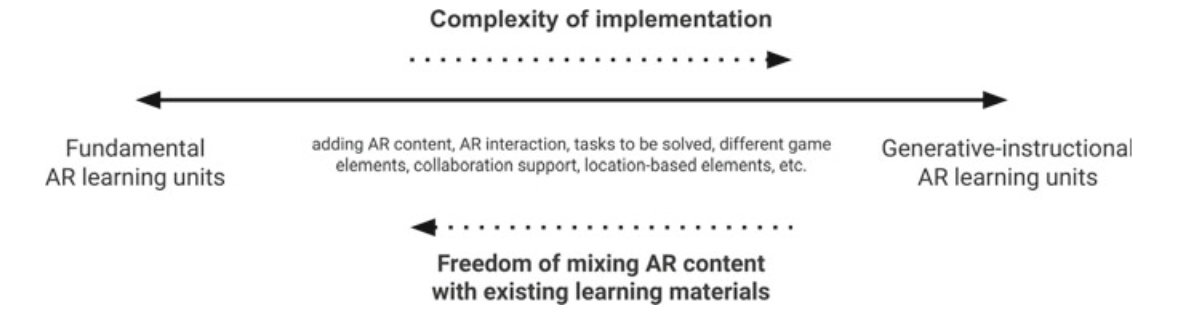
\includegraphics[width=1.0\textwidth]{Abbildungen/ar-object-continuum.png}
\caption[Komplexitätskontinuum von AR-Objekten]{Das Komplexitätskontinuum von AR-Objekten. (Quelle: \cite[S. 9]{geroimenko:ar-in-education})}
\label{fig:komplexitätskontinuum}
\end{figure}
Generell kann bei AR-Objekten zwischen fundamentalen und generativen AR-Lerneinheiten unterschieden werden, die jeweils eine Ende eines Kontinuums darstellen (vergleiche Abbildung \ref{fig:komplexitätskontinuum}).
Der ausschlaggebende Faktor ist dabei die Komplexität des Objektes, je höher diese ist desto generativer ist die Lerneinheit, aber umso geringer ist die Möglichkeit die AR-Inhalte mit den existierenden Lerninhalten zu verbinden. 
Generative AR-Lerneinheiten stehen also mehr für sich alleine und decken ein größeres inhaltliches Feld ab.
Der Zugriff auf diese fundamentalen AR-Inhalte ist heutzutage bereits sehr einfach und die Entwicklung in der Thematik wird sich vermutlich ähnlich analog zu der Entwicklung der VR-Inhalte, bei welcher die generative Inhalte nach und nach hinzukamen, verhalten.\citep[Kapitel 1.3]{geroimenko:ar-in-education}\\
Die aktuelle Hauptzielgruppe im schulischen Bereich ist dabei die weiterführende Schule. Außerhalb des schulischen Umfeldes kommt AR zur Ausbildung von Fachkräften zum Einsatz. \citep[Kapitel 1.5]{geroimenko:ar-in-education}

\subsection{Entwicklung von Augmented Reality Anwendugen}
Bei der Entwicklung von AR-Anwendungen für den Bildungsbereich müssen nach \citeauthor[Kapitel 1.7]{geroimenko:ar-in-education} die folgenden Punkte betrachtet werden:
\subsubsection{Technologie}
Bei der eingesetzten Technologie muss überlegt werden, welche Geräte die Schüler bereits besitzen und welche alternativ angeschafft werden können. Des weiteren muss bedacht werden, dass die Lehrenden im Umgang mit den neuen Technologie geschult werden müssen.
\subsubsection{AR-Lernerfahrungen}
Unter diesem Punkt verbirgt sich die Entscheidung, was mit der Anwendung erreicht werden soll. Dabei muss zwischen fundamentalen Lerneinheiten, die angeschaut und vom Nutzer manipuliert werden können, und generativen, instruktiven Lerneinheiten, welche verschiedenen Interaktionsmöglichkeiten, Spielelemente, Beteiligungsformen und vieles mehr enthalten,  abgewogen werden. 
\subsubsection{Erstellen von AR-Inhalten}
Dieser Punkt beinhaltet die Tatsache, dass es zwar relativ einfach is simple AR Lernobjekte, wie zum Beispiel 3D-Modelle von echten Objekten basierend auf Fotos, zu erstellen, für komplexere Lernerfahrungen, jedoch aufgrund von mangelnden Werkszeugen, Softwareentwicklungskenntnisse notwendig sind.
\subsubsection{Zielgruppe und Themen}
Augmented Reality kann in einem breiten Feld an Einsatzgebieten, wie Schulen, Museen, Galerien und vielem mehr zu Bildungszwecken eingesetzt werden. Dabei unterscheiden sich jedoch die verschiedenen Anforderungen der einzelnen Gebiete und eine Anwendung sollte mit Absprache der Zielgruppen an die konkreten Anwendungsfälle angepasst sein.

\subsection{Augmented Reality in der Lehre}
\citeauthor{geroimenko:ar-in-education} bewertet zudem den Einsatz und die Chancen von Augmented Reality in verschiedenen Bereichen der Bildung. Dabei wurde unter anderem das folgende herausgearbeitet: 

\subsubsection{Medizin, Naturwissenschaften}
Besonders in der Medizin hat Augmented Reality die Möglichkeit ein ein einzigartiges Bildungstool darzustellen. Dabei gibt es für AR vor allem die folgenden Einsatzmöglichkeiten:
\begin{itemize}
\item Anatomie: Hierbei kann AR von Medizinstudenten dazu genutzt werden die Anatomie des Körpers besser zu verstehen, indem sie 3D Modelle im AR-Bereich bertrachten können.
\item Mentoring: Mit Hilfe von AR ist es möglich das Studenten Prozeduren kennenlernen und erfahren, in denen sie noch nicht geschult sind. 
\item Klinische Fertigkeiten: AR bietet die zusätzlich die Möglichkeit die klinischen Fähigkeiten der Studenten zu verbessern, indem mit ihrer Hilfe klinische Simulationen durchgeführt werden können.
\end{itemize}
In den Naturwissenschaften ist der Haupteinsatzzweck das Visualisieren von Modellen, wie dem molekularen Aufbau eines Stoffes. \citep[Kapitel 7-9]{geroimenko:ar-in-education}

\subsubsection{Geisteswissenschaften}
Ein wichtiges Anwendungsbeispiel für diesen Bereich ist die Erweiterung der Umgebung basierend auf der aktuellen Position des Nutzers  durch AR. Dadurch lassen sich beispielsweise Zusatzinformationen zu historischen Gebäuden anzeigen und es ist möglich dem Nutzer einen Eindruck zu vermitteln, wie ein Ort in der Vergangenheit einmal aussah. \\
Im Bereich des Lernens einer Fremdsprache, bietet AR die Möglichkeit das konventionelle Lernen im Klassenzimmer um eine virtuelle Welt erweitern, um die Motivation der Lernenden zu steigern. \citep[Kapitel 11-12]{geroimenko:ar-in-education}

\subsubsection{Umweltpädagogik}
Im Bereich der Umweltwissenschaften kann Augmented Reality beispielsweise für eine Umweltbildung im Freien genutzt werden. Dabei bietet AR die Möglichkeit die Komplexität der Umgebung aus verschiedenen Perspektiven zu visualisieren, detaillierte und wissenschaftliche Informationen anzuzeigen oder das \glqq unsichtbare\grqq{} sichtbar zumachen. \\
Die Augmented Reality kann also dazu genutzt werden, dem Lernenden eine andere Perspektive auf das Sichtbare zu ermöglichen, in dem es Parameter, wie die Zeit (Vergangenheit, Zukunft), die Skalierung (mikroskopische Sicht, Vogelperspektive) oder die Wahrnehmbarkeit (Unsichtbares enthüllen, Sichtbares verdecken), verändert.\\
Auch in der Archäologie kann AR eingesetzt werden. In diesem Bereich dient es als Forschungsinstrument für die Rekonstruktion und Interpretation. \citep[Kapitel 17]{geroimenko:ar-in-education}

\subsection{Weitere Anwendungsbeispiele}
Im Rahmen des Buches wurden zudem auch verschiedene, weitere Anwendungsfälle für Augmented Reality im Bildungsbereich vorgestellt, die im Folgenden noch einmal aufgegriffen werden. 

\subsubsection{Webbasierte Augmented Reality Anwendung}
Ein Anwendungsbeispiel ist eine konkrete Online-Plattform zur verbesserten Lernerfahrung. Die Anwendung beruht auf \glqq durchsichtige\grqq{} Marker, die in ein Bild eingefügt werden konnten. Wurde der Marker innerhalb eines Bildes erkannt wurde ein zugeordnetes, interaktives 3D-Modell angezeigt. \citep[Kapitel 3]{geroimenko:ar-in-education}

\subsubsection{FeDiNAR}
Das FeDiNAR-Projekt hat das Ziel Fehler mit Hilfe von Augmented Reality zu einer Lernmöglichkeit umzuwandeln. Das Konzept beruht darauf Fehler nicht durch den Ausbilder zu verhindern, sondern sie zuzulassen. Dieses soll den Ausbilder möglich sein, indem die Auszubildenden zwar an echten Maschinen arbeiten, die Auswirkungen ihrer Handlungen dabei jedoch lediglich in der Augmented Reality dargestellt werden. 
\citep[Kapitel 5]{geroimenko:ar-in-education}

\section{A Systematic Review of Learning through Mobile Augmented Reality}
In der wissenschaftlichen Arbeit von \citeauthor{hedberg:review-ar-learning} \citep{hedberg:review-ar-learning} wurde mit Hilfe einer systematischen Literaturauswertung eine Einschätzung des Einsatzes von Augmented Reality zu Bildungszwecken vorgenommen. \\
Dabei wurde die Relevanz einzelner Einsatzgebiete anhand der Anzahl an Veröffentlichungen zum jeweiligen Thema gemessen.\\ Die Veröffenntlichungen stammen dabei aus den Datenbanken \glqq IEEE Xplore\grqq , \glqq Elsevier\grqq{} und der \glqq ACM digital libary\grqq{} und wurden über Schlüsselwörter herausgesucht. Die Ergebnisse der Suche wurden im Anschluss noch gefiltert und kategorisiert, um irrelevante Veröffentlichungen auszuschließen.
\subsection{Ergebnisse}
Anhand der gesammelten wissenschaftlichen Arbeiten kam die Studie zu den folgenden Ergebnissen in den für diese Arbeit relevanten Kategorien:

\subsubsection{Bildungsniveau}
Diese Kategorie zielte darauf ab die Zielgruppen der AR-Systeme herauszufinden. Dabei kam die Studie zu dem Ergebnis, dass die meisten Systeme (fast 50 \%) bezogen auf das amerikanische Bildungssystem für die Universität geschaffen wurden. Mit einem deutlichen Abstand folgt die Grundschule, die Junior High School, die High School und die Vorschule. \citep[S. 78]{hedberg:review-ar-learning}

\subsubsection{Mobiles Endgerät}
In dieser Kategorie ging es darum herauszufinden, welches die meist genutzten Endgeräte für Augmented Reality im Bildungsbereich darstellen. Hierbei kam heraus, dass das Handy bzw. das Smartphone (43,84 \%) gefolgt von dem Tablet (27,40 \%) diese Kategorie dominieren, wobei ebenfalls 27 \% der wissenschaftlichen Arbeiten keine spezifische Plattform angaben. \citep[S. 80]{hedberg:review-ar-learning}

\subsubsection{Unterrichtsfach}
Diese Kategorie untersuchte die fachliche Ausrichtung der Augmented Reality und kam zu dem Ergebnis das die Systeme vor allem in den Naturwissenschaften genutzt werden. Darauf folgen mit signifikantem Abstand die Sprachen, Geschichte und Technik. \citep[S. 81]{hedberg:review-ar-learning}

\subsubsection{Lernerfolge}
Hier bei wurden Studien untersucht, die sich mit dem pädagogischen Nutzen von Augmented Reality beschäftigt haben. Dabei kamen von 73 Studien lediglich zwei nicht zu dem Ergebnis, dass AR einen positiven Einfluss auf das Lernen besitzt.\\
Allgemein stellten 45 Veröffentlichungen (54,88 \%) eine erhöhte Motivation und ein verbessertes Engagement fest. 28 Studien (34,15 \%)konnten verbesserte Lernergebnisse bei den Studenten aufzeigen.  \citep[S. 81-82]{hedberg:review-ar-learning}

\subsubsection{Pädagogische Methoden}
In der letzten Kategorie, wurden die Einsatzarten von Augmented Reality im Bildungsbereich untersucht und das Ergebnis erarbeitet, dass die drei Hauptanwendungsmethoden das interaktive, das forschungsbasierte und das kollaborative Lernen sind. \citep[S. 82]{hedberg:review-ar-learning}

\section{Augmented Reality in Education}\label{sec:billinghurst-ar-education}
\citeauthor{billinghurst:ar-in-education} untersuchte in seiner wissenschaftlichen Arbeit \citep{billinghurst:ar-in-education} den Einsatz von Augmented Reality im Bildungsbereich.\\
Dabei geht er in den folgenden drei Unterkapiteln auf unterschiedliche Eigenschaften der AR im Bildungsbereich ein.

\subsection{Nahtlose Interaktion}
\citeauthor{billinghurst:ar-in-education} führt hier auf, dass Schüler besser zusammenarbeiten, wenn sie sich gemeinsam auf einen Arbeitsplatz fokussieren. Dieses ist bei computerbasierten Lernen schwierig um zusetzten, da sich jeder auf den Bildschirm vor sich fokussiert. Dadurch fehlt eine wichtige Eigenschaft, die die Kommunikation in der Gruppe verbessert: die gegenseitige Sichtbarkeit. Wenn Schüler gleichzeitig das Objekt der Diskussion und ihre Diskussionspartnern sehen, werden auch die nichtverbalen Gesprächsmerkmale, wie Gesten oder die Mimik wahrgenommen. Diese Merkmale bilden einen essentiellen Teil der menschlichen Kommunikation. \\
Durch den Einsatz von Augmented Reality können diese Eigenschaften bei behalten werden und trotzdem gleichzeitig computerbasierte Inhalte angezeigt werden. \citep[S. 2-3]{billinghurst:ar-in-education}

\subsection{Greifbare Schnittstelle}
Hier führt \citeauthor{billinghurst:ar-in-education} auf, dass im Bildungsbereich physische Objekte dazu genutzt werden Bedeutung von theoretischem Wissen zu übermitteln, in dem sie die Eindrücke des Schülers, durch ihre Erscheinung, ihre physkalischen Eigenschaften, ihren räumlichen Beziehungen und der Fähigkeit, die Aufmerksamkeit zu fokussieren, verstärken.\\
Diese Eigenschaften lassen sich zu großen Teilen auch auf die virtuellen Objekte in der Augmented Reality beziehen. Auf Grund der direkten Beziehungen zwischen der virtuellen Objekten und der Augmented Reality ist zum Beispiel eine physikalisch basierte Interaktion mit den computergenerierten Objekten möglich. \citep[S. 3]{billinghurst:ar-in-education}

\subsection{Übergangsschnittstelle}
Im dritten Abschnitt bezieht sich \citeauthor{billinghurst:ar-in-education} auf das bereits in Kapitel \ref{sec:ar} eingeführte RV-Kontinuum und führt an, dass man mittels AR den Nutzer entlang des Kontinuums in die virtuelle Welt führen kann. Besonders Kinder können so in die Seiten eines Buches eintauchen und die Fantasie Realität werden lassen. Dadurch werden aus statischen Unterrichtsbüchern dynamische interaktive Umgebungen. \citep[S. 3-4]{billinghurst:ar-in-education}


\section{Benefits of Augmented Reality in Educational Environments}\label{sec:diegmann-benefits-ar}
In dem Artikel \citep{diegmann:benefits-ar} von \citeauthor{diegmann:benefits-ar} werden die Vorteile von Augmented Reality betrachtet. \\
Dabei wurde eine systematische Evaluation von Augmented Reality anhand der Veröffentlichungen zu diesem Thema durchgeführt. \\
Im folgenden werden einmal die Kernaussagen zusammengefasst.

\subsection{Vorteile}
Basierend auf der Literatur stellte der Artikel zunächst in den folgenden Bereichen positive Effekte der Augmented Reality fest:

\subsubsection{Geisteszustand}
In verschiedenen Veröffentlichungen wurde eine Verbesserung der Motivation festgestellt. Dieses umfasst ein erhöhtes Engagement und Interesse gegenüber den Lerninhalten und der Technologie.\\
Des weiteren wurde auch eine Steigerung der Aufmerksamkeit und der Konzentration, bezogen auf die Inhalte mit denen die Lernenden konfrontiert wurden, festgestellt.\\
Zu dem verbesserte sich auch die Zufriedenheit der Schüler bezüglich der Bildungsfortschritte und des Lernprozesses. 
\citep[Kapitel 4.1]{diegmann:benefits-ar}

\subsubsection{Lehrkonzept}
Das Lehrkonzept verbessert sich durch AR  dahingehend, dass ein schülerzentriertes Lernen ermöglicht, wodurch das unabhängige, eigenverantwortliche Lernen der Schüler, sowie die Fähigkeit Wissensinhalte aufzunehmen verbessert wird.\\
Auch eine Verbesserung des kollaborativen Lernens kann durch AR erreicht werden. Dabei kann Schülern durch AR die Möglichkeit zur gemeinsamen Problemlösung und Kommunikation gegeben werden.
\citep[Kapitel 4.2]{diegmann:benefits-ar}

\subsubsection{Darstellung}
Auch die Darstellung von Lerninhalten kann mit Hilfe von AR-Anwendungen verbessert werden. So können AR-Inhalte einen höheren Detailgrad ermöglichen und die Zugänglichkeit von Lerninhalten und die Interaktivität mit diesen Inhalten. verbessern. Besonders die neuen Interaktionsmöglichkeiten unterstützen ein Lernen durch eigene Erfahrungen.
\citep[Kapitel 4.3]{diegmann:benefits-ar}

\subsubsection{Lerntyp}
Ein weiterer Vorteil ist die Verbesserung der Lernkurve dar. Schüler die mit Hilfe von Augmented Reality Unterrichtsinhalte erfassen konnten lernten schneller und einfacher als Schüler ohne diese Möglichkeit.\\
Auch eine Verbesserung der Kreativität, der Wissensaufnahme und der Problemlösung konnte in verschiedenen Veröffentlichungen festgestellt werden.
\citep[Kapitel 4.4]{diegmann:benefits-ar}

\subsubsection{Verständnis}
Dieser Bereich bezieht sich auf das Wissen, das durch Augmented Reality erlangt werden kann.\\
Dabei kann, neben einem deutlich gesteigertem, räumlichen Verständnisses, auch eine Steigerung des Gedächtnisses beobachtet werden. So konnten Schüler mit Hilfe von AR sich besser an Inhalte erinnern. \\
\citep[Kapitel 4.5]{diegmann:benefits-ar}

\subsection{Zuordnung der Vorteile zu verschiedenen Anwendungsarten}
In einem zweiten Schritt ordnet der Artikel, die im vorherigen Kapitel definierte Vorteile bestimmten AR-Anwendungsarten zu. Diese Anwendungsarten werden im folgenden einmal betrachtet:

\subsubsection{Entdeckungsbasiertes Lernen}
Bei entdeckungsbasierten Anwendungen erhält der Benutzer \glqq Informationen über einen realen Ort, während er gleichzeitig das interessierende Objekt betrachtet\grqq{} \citep[Kapitel 2.2]{diegmann:benefits-ar} \\
Bei Art von Anwendungen konnte vor allem eine Verbesserung der Lernkurve und des Geisteszustandes bei den Lernenden beobachtet werden. Insgesamt deckt diese Kategorie die meisten Vorteile im Vergleich zu den anderen Anwendungsarten ab.
\citep[Kapitel 5]{diegmann:benefits-ar} \\
\subsubsection{Objektmodellierung}
Diese Gruppe beschreibt Modellierungsanwendungen, die mit Hilfe von Augmented Reality dem Nutzer direktes Feedback zur Optik der modellierten Objekte geben. \citep[Kapitel 2.2]{diegmann:benefits-ar} \\
Bei dieser Anwendungsart konnte in der Literatur eine erhöhte Motivation, eine verbesserte Zufriedenheit und eine angestiegene Lernkurve bei den Studierenden festgestellt werden. Jedoch konnte trotz der starken Interaktion mit der Augmented Reality, keine Artikel gefunden werden die von einer verbesserten Interaktivität oder Kreativität berichteten. \citep[Kapitel 5]{diegmann:benefits-ar}

\subsubsection{AR-Bücher}
AR-Bücher bezeichnen Bücher, die durch Augmented Reality angereichert werden. Dabei stellen sie dem Leser 3D-Darstellungen der Lerninhalte zur Verfügung, wenn dieser das Buch mit Hilfe von speziellen, AR-fähigen Geräten betrachtet. \citep[Kapitel 2.2]{diegmann:benefits-ar}\\
Die wenigsten Veröffentlichungen konnten diese Kategorie abdecken und dem entsprechend wenig Vorteile wurden in den Arbeiten herausgestellt. Lediglich sechs der zuvor definierten Vorteil waren in der Literatur wieder zu finden. \citep[Kapitel 5]{diegmann:benefits-ar}

\subsubsection{Fähigkeitentraining}
Diese Kategorie umfasst Anwendungen die das Trainieren spezieller Fähigkeiten trainieren, in dem sie die Abläufe, Trainingsobjekte oder Ähnliches bereitstellen. \citep[Kapitel 2.2]{diegmann:benefits-ar} \\
Anwendungen die in den Bereich des Fähigkeitentrainings fallen haben in der Literatur die meisten Erwähnungen eines verbesserten Verständnisses. Des weiteren wird häufig eine Verbesserung der Lernkurve erwähnt. \citep[Kapitel 5]{diegmann:benefits-ar}

\subsubsection{AR-Spiele}
In dieser Gruppe befinden sich Video-Spiele, die mit Hilfe von Augmented Reality dem Schüler Lerninhalte vermitteln sollen. \citep[Kapitel 2.2]{diegmann:benefits-ar} \\
Die Vorteile von AR-Spielen liegen laut der Literatur vor allem im Bereich Bereich des Geisteszustands, der Lernkurve und der Zugänglichkeit zu den Lerninhalten. \citep[Kapitel 5]{diegmann:benefits-ar}



\section{A Systematic Review of 10 Years of Augmented Reality Usability Studies}
In dem Artikel \citep{dey:review-of-ar-studies} von \citeauthor{dey:review-of-ar-studies} wird eine Auswertung von verschiedenen Studien, die sich mit dem Einsatz von Augmented Reality beschäftigen, durchgeführt. Dabei wird ein Überblick über die Veröffentlichungen aus den Jahren von 2005 bis 2014 gegeben.\\
Insgesamt wurden in dem Artikel die folgenden Ergebnisse herausgestellt.

\subsection{Display}
Allgemein betrachtet stellen Head Mounted Displays (HMD, deutsch: \glqq Am Kopf befestigter Bildschirm\grqq ) und Hand-Held Displays (HHD, deutsch: \glqq Handdisplay\grqq ) die meistgenutzten Wiedergabegeräte dar.\\
Im Bildungsbereich kommen HMDs hingegen kaum zum Einsatz. Hier dominieren vor allem HHDs, gefolgt von Desktopbildschirmen und  verschiedene Arten von großformatigen Anzeigen. \citep[Kapitel 3.7]{dey:review-of-ar-studies}

\subsection{Bildungsbereich}
Alle Studien die sich mit dem Einsatz im Bildungsbereich beschäftigten, bezogen sich auf eine Methode des Unterrichtens oder des Lernens. Basierend auf den Schlüsselwörtern der Studien sind vor allem das Lernen, die Interaktivität, die Nutzer und die Umgebung relevant für den Bildungsbereich.\\
Eine Studie von Fonseca u. a, die im Rahmen des Artikels genauer betrachtet wurde, untersuchte den Einsatz einer Smartphone basierten AR-Anwendung, die zur Visualisierung von 3D-Modellen genutzt werden kann, in einem schulischen Umfeld. Dabei beobachteten sie eine erhöhte Motivation und eine Verbesserung der akademischen Leistungen. \\
Diese Anwendung stellt nur ein Beispiel der untersuchten Einsatzmethoden von AR dar. Insgesamt wurden in den Studien die verschiedensten Einsatzmöglichkeiten von Anwendungen untersucht. Darunter waren beispielsweise Applikationen, die Personen mit Amputationen im Umgang mit Prothesen schulen, Anwendungen, die kognitiv beeinträchtigte Menschen bei der Erwerbung von beruflichen Fähigkeiten unterstützen oder AR-Systemen, welche zum Unterrichten der historischen Seiten einer Stadt genutzt werden können. \\
Auf dieser Grundlage betonen die Autoren, die Variabilität in den Einsatzmethoden, die im Bildungsbereich genutzt werden können. \citep[Kapitel 4.2]{dey:review-of-ar-studies}


\section{Augmented Reality als Bildungsenhancement?}
In dem Artikel \citep{damberger:ar-bildungsenhancement} von \citeauthor{damberger:ar-bildungsenhancement} wird die Frage thematisiert, ob Augmented Reality die Bildungsprozesse verbessern kann. Eine solche Verbesserung, die auf dem Einsatz von Technologien beruht, bezeichnet der Autor als Bildungsenhancement. \\
Dabei wird jedoch betont, dass mit dem Bergriff nicht die Verbesserung der Bildung selbst gemeint ist. Dieses ist mit Hilfe von AR ebenso wenig möglich, wie durch einen gesteigerten Konsum an (Fach-)Literatur, so der Autor.
\begin{quote}
\glqq Bildungsenhancement soll vielmehr einen durch Technik ermöglichten besonderen Zugang zur Welt beschreiben, der reflexive Prozesse eröffnet, in deren Folge ein Mehr an Bildung möglich werden kann.\grqq \citep[S. 5]{damberger:ar-bildungsenhancement}
\end{quote}
Im Laufe des Artikels betrachtet der Autor, die oben genannte Frage aus einer philosophischen Sicht.

\subsection{Augmented Reality als Erweiterung der Realität}
Augmented Reality bietet dem Menschen die Möglichkeit seine Umgebung mit virtuellen Objekten zu ergänzen. Dieses Fähigkeit bietet großes didaktisches Potential, indem sie es dem Menschen erlaubt den realen Objekten, mit dem sie arbeiten um Informationen zu erweitern.\\
Da diese Informationen nicht nur subjektiver Art sein müssen, sondern auch objektive Eindrücke und Erfahrungen anderer Menschen repräsentieren können, erlaubt es Augmented Reality mehr Welt zu erfassen und diese auf eine andere Weise wahrzunehmen. Dadurch \glqq enhanced\grqq{} AR die Bildung zwar nicht unbedingt, bietet aber einen anderen Zugang zu den Repräsentationen der Welt und stellt somit eine Erweiterung der Bildung dar. \citep[S. 22-23]{damberger:ar-bildungsenhancement}


\section{Offener Geschichtsunterricht mit Augmented Reality}
Der Artikel \citep{buchner:ar-geschichtsunterricht} von \citeauthor{buchner:ar-geschichtsunterricht} beschäftigt sich mit einem Unterrichtsszenario zum Einsatz von Augmented Reality im Fach Geschichte, Sozialkunde und Politik. 
Grundlage des Artikels ist die Problematik, dass für einen kompetenzorientierten im Vergleich zum inhaltsorientierten Unterricht, eine intensive und aktive Auseinandersetzung mit dem Unterrichtsthemen notwendig ist und eine reine Wissensrezeption nicht mehr ausreicht.\\ 
Des weiteren wird angezweifelt, dass der klassische Lehrervortrag zur Kompetenzvermittlung nicht geeignet ist, auch wenn er im folgenden noch einen Großteil der Unterrichtszeit einnehmen wird. Der Artikel stellt hier heraus, dass die Methodenvielfalt ein wichtiges Qualitätsmerkmal der Wissensvermittlung darstellt und das beim Einsatz von digitalen Medien nicht das Tool im Mittelpunkt stehen sollte, sondern das didaktische Problem.\\

\subsection{Lehren und Lernen mit Augmented Reality}
Eine Einsatzmöglichkeit von Augmented Reality stellt das Unterstützen von authentischen Geschichten dar, so wird in dem Artikel das Beispiel angebracht, dass in einem Museum in Salzburg mit Hilfe von Markern, die in den Schaukasten angebracht sind, animierte Figuren im AR-Bereich angezeigt werden können, die den Besuchern Geschichten über beispielsweise das Leben der Kelten erzählen. \\
Laut verschiedener Studien hat Augmented Reality positive Auswirkungen auf den kognitiven Wissenserwerb, die Motivation, das Interesse, aber auch auf überfachliche Kompetenzen, wie das Suchen, Organisieren und Evaluieren von Informationen. \\
Des weiteren wurden Studien heran gezogen, die das größte Potential von AR in der Gestaltung authentischer, flexibler und mobiler Lernumgebungen sehen. \citep[Kapitel 3]{buchner:ar-geschichtsunterricht}

\subsection{Anwendung im Geschichtsunterricht}
Im Rahmen des Artikels wurde ein beispielhafter Einsatz in der dritten Klasse eines Wiener Gymnasiums im Fach Geschichte getestet.\\
Dafür wurden Videos zu den entsprechenden inhaltlichen Thematiken gedreht, dessen Startbilder anschließend als Marker fungierten. Haben die Schüler nun diese Bilder eingescannt wurden sie so mit dem Video überlagert als ob das Bild zum Leben erwachen würde. \\
Am Ende des entsprechenden Videos wurde jeweils einen Aufgabe für die Schüler eingebaut, so öffnete sich beispielsweise automatisch ein Quiz. \citep[Kapitel 4]{buchner:ar-geschichtsunterricht}

\subsection{Fazit}
\citeauthor{buchner:ar-geschichtsunterricht} konnte in beiden Klassen positive Einflüsse der AR-Lernumgebung auf das Interesse, die wahrgenommene Kompetenz und Wahlfreiheit feststellen.\\
Das Ganze Experiment traf auch über das Projekt hinaus auf Anspruch, sodass sich an dem entsprechenden Gymnasium anschließend Lehrer zusammengeschlossen haben um weitere Schülerzentrierte Lernumgebungen zu entwerfen. \citep[Kapitel 5-6]{buchner:ar-geschichtsunterricht}


\section{Atlas der Humananatomie}\label{sec:atlas-humananatomie}
Visible Body stellt mit der Anwendung \glqq Atlas der Humananatomie 2020\grqq{} eine Anwendung zur Visualisierung von anatomischen Modellen bereit. \todo{zitieren?} Diese steht auch Studenten der Universität Oldenburg über den Bibliothekszugang zur Verfügung und kommt im medizinischen Bereich zum Einsatz. \\
\subsection{Anwendung}
Innerhalb der Applikation stehen dem Nutzer verschiedene anatomische Modelle zur Auswahl. Wird eines dieser Modelle ausgewählt wird es zunächst vor einem eintönigen Hintergrund angezeigt. Allerdings besteht zusätzlich die Möglichkeit das Modell im Augmented Reality Bereich darzustellen (siehe \ref{fig:atlas-skelett)}. \\
Mit Hilfe von Gesten kann der Nutzer mit dem Modell interagieren.
\begin{figure}[h!]
\centering
\includegraphics[width=0.8\textwidth]{Abbildungen/app-atlas-skelett.png}
\caption[Atlas der Humananatomie]{Die Darstellung des menschlichen Skeletts in der Anwendung \glqq Atlas der Humananatomie 2020\grqq . (Quelle: Screenshot aus der Anwendung \glqq Atlas der Humananatomie 2020\grqq )}
\label{fig:atlas-skelett}
\end{figure}



